\documentclass[a4paper]{article}
% Utility function -> Maximize QoE - find the optimal balance between QoE and best usage of resources
\usepackage[english]{babel}
\usepackage[utf8]{inputenc}
\usepackage{amsmath}
\usepackage{graphicx}
\graphicspath{ {C:/images } }
\usepackage[colorinlistoftodos]{todonotes}

\title{An SDN-approach for QoE management of Multimedia services using autonomous behavior}

\author{Elisavet,Luigi,Alex}
% * <elisavetgrig@gmail.com> 2016-07-08T09:25:36.950Z:
%
% > Elisavet,Luigi,Ale
%
% ^.

\date{\today}

\begin{document}
\maketitle
\begin{abstract}
Your abstract.
\end{abstract}

\section{Introduction}

In  future networks will exist a huge explosion of traffic especially with the increased use of diverse devices with Internet-of-Things(IoTs), and this could lead to inefficient utilization of radio resources. Also, the large and increasing varieties of proprietary network hardware appliances are going to increase the complexity and the upgrade costs of a network. Furthermore, issues such as lack of flexibility and agility are going to be observed, especially in case of a new service. It will be difficult and takes too long to launch a new service. %To lunch what?this is sentence is not clear to me\\

Moreover, in today`s competitive environment users have the option to choose from a variety of service providers. Therefore, the service availability is not enough anymore. Thus, they must deliver the services in such a way that users will fully enjoy a rich experience at a logical price improving the Quality of Experience (QoE). QoE is defined as the measure of how well a system or an application meets the user`s expectations. This is different from Quality of Service (QoS), which is focusing on measuring performance from a network perspective. With no doubt,  QoE is directly related to QoS, but the challenge for a service provider is to have the right set of mechanisms to control it [1] in order to have greater impact to his balance sheets reducing the users` churn. \\

A main issue in future networks is the management of QoE. The QoE estimation in future networks services will require per application analysis in which the main properties that can impact user-perceived quality are determined. The monitoring and measuring of QoE is a different thing from the maximization of it. The maximization of QoE requires early detection of potential QoE-affecting problems and solves them as soon as possible and in the same time prioritizes them, in order to tackle with highest impact problems in terms of potential revenue. [1] \\

Thus , the aim of this paper is to develop an SD-based approach for QoE management of future multimedia services.In order to meet this goal, this paper develop a flexible, an efficient and scalable architecture with autonomous behavior in order to succeed high level of QoE in future networks.

SDN and   three principles: (i) Network Softwarization using technologies such as Software-Defined Networks (SDN) and Network Function Virtualization (NFV), (ii) unbundling using software/hardware decoupling and control/user plane separation, and (iii) Open using open source software and open interfaces.//
Flexibility, scalability and autonomous behavior objective can be achieved by Network Softwarization [NetSoft2015]. Network softwarization is a transformation trend to design, implement, deploy, manage and maintain network equipment and network components by software programming. Network softwarization provides  distributed virtual platforms which can excute any network function and networked services  as applications on Virtual Machines which are allocated, managed and moved dynamically on general purpose Hardware//
This paper adopts the principles and the use of of SDN and NFV in the development of QoE management approach for future multimedia services in the next generation networks.//

In SDNs, the network control is separated from the user plane and thus we are able to manage the network resources regarding the design, delivery and operation of network services in a scalable, flexible and dynamic way. Furthermore, the NFV allows virtualization of software-based network functions. There is no longer need to install and manage dedicated hardware devices for networking and service functions.
%For network operators, SDNs and NFV have a potential significant reductions of CAPEX and OPEX and aim on softwarization of everything everywhere in order to meet various network management and service objectives.
%[ITU T13-SG13].//is this a reference to a previous sentence or the next sentence.
%ITU T13-SG13.However, in the same time, this paper implements distributed controllers in SDN with autonomous behaviorwe in order to avoid the main problem of SDNs regarding the centralized controller, which is a single point of failure.// 

In fact, there is a need for intelligent control algorithms that coordinate the different autonomous entities [3]. This is achieved through control loops that dynamically configure the network but are deployed in a loosely coupled distributed environment where multiple autonomous entities work together to jointly manage the network and form an end-to-end QoE optimization from the service originator up to the end customer[4]. \\

Multimedia applications can be decomposed into a set of tasks. Some tasks can run in parallel way and some other task must be processed serially. The goal of task-level scheduling is to assign tasks to VMs so that the total execution time can be minimized. This kind of scheduling is performed in a hierarchical way.\\

An effective task-scheduling can match demands of tasks with resource provisioning of VMs and improve QoE. Although, it is a challenge to achieve this regarding some issues. Firstly, there are some priority constraints, which are the priorities between the tasks. (example figure with the linear DAG). Also, the multimedia applications have different operation structures. Generally, there are 3 basic structures: sequential, parallel and mixed structures. In this paper, we are focusing on sequential structures, in which the task are executed in a serial order, with one task starting after a previous task has completed. In parallel structures, the task can be performed concurrently and the mixed are combined both sequential and parallel structures. It is a challenge to find one effective scheduling scheme for different structures, that why currently we are focusing only in the sequential. Furthermore, another challenge is the assignment of a task to the best suitable VM because every VM has different resource capacities. \\

In current paper, we are apply a multimedia task-level scheduling using Software Defined Networks and Network Function Virtualization in order to improve the overall Quality of Experience.  




\section{State-of-the-Art Section}

 The network resource allocation is a major problem of multimedia communications. In order to address this problem, a cross-layer approach has been proposed in [7]. There have been conducted many studies regarding optimization of network resource allocation for wireless video delivery but most of them are focusing on throughput maximization [8]. Although, in real-time applications such as video streaming, there are dynamic changes of the application requirements (e.g. delay, packet loss, data rate, etc.) thus the QoE optimization that based on throughput is not the optimal solution with respect to the user-perceived quality. [7] Note that, initially, the QoE-based optimization proposed for elastic application such as file transfers, which captures the user`s satisfaction as a function of data rate using a concave utility function. [9]\\

In [7], the authors apply a QoE-based optimization framework in order to allocate efficiently the network resources for video delivery. The aim from network operator`s view is to allow the maximum number of users to join the system and in the same time to keep a good level of service quality. In order to do that, the operator has the ability to set a policy. The operator sets a “Target mean MOS” for all users and this leads to a significant network resource saving. These resources could be used in the future from other users or could be used for the support of high-demand applications. \\

\section{Framework}
In this paper, our target is to improve the overall QoE in case of adaptive video streaming application using NFV and SDN technologies. 
Numerous challenges may be identified related to the issue of QoE optimization. The initial concern involves modeling QoE for a video streaming service in terms of identifying QoE influence factors and their relationship to QoE Metrics. But first we are going to present the framework that we based in order to develop our model. Our idea is to improve each parameter in these categories in order to improve the overall QoE. Thus, our framework is based on the classification of ARCU model [arcuModel]. 
In this model, the Influence Factors  categorized in 4 categories: Application-related, Resource-related, Context-related and User-related. Regarding our service the related parameters in these categories are the following: 

\begin{enumerate}
\item \textbf{Application-related} 
We consider video parameters such as codec, bitrate and bandwidth, in order to improve the quality of the content and the response time of the service. \\
% how we can change the codec? how we can improve this? % 
% how we can improve the bitrate and the bandwidth? %

\item \textbf{Resource-related} 
We consider the QoS parameters such as delay and packet loss. Our target is to maximize the QoS in order to improve the reliability of the service in question. \\
% function to maximize the QoS %

\item \textbf{Context-related} 
We consider the costs of virtual machines. Our target is to minimize the cost of the virtual machines in order to improve the acceptability. \\
% function - execution cost component - elisavet% 
\item  \textbf{User-related} 
We consider the Mean Opinion Score(MOS) as metric in this case. Our target is to maximize the MOS, thus to improve user`s satisfaction.\\
% QoS - MOS -> estimate MOS by correlation with QoS%

\end{enumerate}
In order to improve the overall QoE we should improve all the above parameters with specific techniques or functions. Because the quality optimization problem consists of maximizing a multidimensional quality function. Thus, in this case, we establish the quality levels and then we optimize them. 

\section{Problem Formulation}
We formulate the problem of dynamic task allocation in an adaptive video streaming scenario considering QoE influence factors in order to improve the overall QoE. Regarding QoE , we consider many influence factors as we discussed in previous section, that influence the video quality perceived by the end-user.  The proposed architecture is based on Network Function Virtualization (NFV) and Software Defined network (SDN) technologies. \\

Different applications have different requirements and different parameters and a variety of tasks have to be executed. Each application can be divided into smaller tasks that can be assigned to different Virtual Machines (VMs) in order to be executed. VMs are installed in different network devices (NDs) each one implementing only one Virtual Function (VF), as illustrated in Figure~\ref{fig:networkmodelnfvsdn}. Each network device denoted as \textit{N} and each NF as \textit{F}. There are \textit{j} types of a NF instances. Each type have different price and capabilities. \\ 

%we should define the NFs%
Due to the heterogeneous characteristics, some VMs can perform the same task faster than others or the cost may be different. The Negotiation and Execution (NaE) [Old TAN] [10] algorithm is used to allocate the tasks to suitable VMs. NaE algorithm includes negotiations between the network devices to determine task assignments. When a network device receives data, it decides if it is going to perform a task or not. \\

\begin{figure}[!ht]
  \caption{Network Model NFV/SDN view}
  \centering
    \includegraphics[width=0.9\textwidth]{nfvmodel3.png}
    \label{fig:networkmodelnfvsdn}
\end{figure}

\section{Task Model}
There is an video application defined as \textit{app} in a set of \textit{K} applications. This application is described as a Directed Acyclic Graph (DAG) of tasks. In order to declare the priority constraints among different multimedia tasks, we present a DAG in figure~\ref{fig:generictasks} . A DAG is a directed graph with no path that starts and ends at the same vertex. Also, it can be denoted as: DAG = $G$ = (X,E).\textit{X} is the set of vertices and \textit{E} is the set of edges. 

\begin{figure}[!ht]
  \caption{Example of a linear DAG}
  \centering
    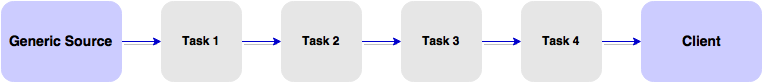
\includegraphics[width=0.9\textwidth]{generic_tasks2.png}
    \label{fig:generictasks}
\end{figure}

We suppose that a multimedia application can be decomposed into $\lambda$ tasks. Each node in the DAG, represents a task. 
Thus X= {X1, X2, ... X$\lambda$} represents the set of the tasks. Each edge in the DAG is characterizing the priority constraint between two tasks, e.g. the Task 3 cannot be executed until Task2 has finished. Figure ~\ref{fig:adaptivestreaming} illustrates the DAG of the media streaming content task chain. In this case, the delivery chain includes 4 task: Transcoding, Encapsulation, Encryption and Origin Server[11]. Thus, each one of these tasks should be executed by a VM.

\begin{figure}[!ht]
  \caption{DAG for adaptive media streaming}
  \centering
    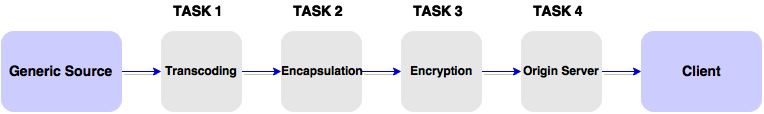
\includegraphics[width=0.9\textwidth]{adaptivestreamingtaks.png}
    \label{fig:adaptivestreaming}
\end{figure}

\section{Network Model}
The network includes two types of nodes, the Network Devices (NDs) and the Network Functions (NFs). Each Network Device (ND) consists of many Virtual Machines (VMs). Each VM implements one Virtual Function (VF) %we should specify which Functions%. 
We declare that $s_j^\lambda$ = 1, if the $X_\lambda$ is assigned to a \textit{j} VM, otherwise it is equal to 0. \\

At the top of the hierarchy is an Application in Management Plane, which manages the network devices via the SDN Controller.
The negotiations are performed among vMs in the same ND, thus there are no multi hop negotiations. Thus, there is no communication between VMs belonging to different NDs, in order to reduce the overhead caused by negotiations. The Network model is illustrated in Figure~\ref{fig:networkmodel}.

Suppose that there are \textit{J} types of VF instances. Each task can be served by specific type VF instance, because different types of VF instances have different price rates and resource capabilities, which leads to different execution time. 
We denote  $t^\lambda_j$ as the execution time by using type \textit{j} VM instance to execute the task $X_\lambda$
We assume that each task can only be assigned to one VM instance for execution. Thus, our purpose is the dynamic assignment of the tasks to VMs in order to improve the QoE perceived from the end-user considering QoE influence factors. 


\begin{figure}[!ht]
  \caption{Network Model}
  \centering
    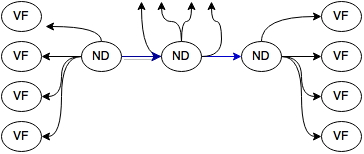
\includegraphics[width=0.9\textwidth]{networkmodel3.png}
    \label{fig:networkmodel}
\end{figure}


A binary vector $s(i) = [s(i, \lambda)]$ for $\lambda \in Tasks$ can be assigned to each node \textit{i} in the network. The state $s(i, \lambda)$ is a boolean value representing the current state of node \textit{i} corresponding to task $\lambda$, i.e $s(i,\lambda) = 1$ when node \textit{i} performs task $\lambda$. The \textit{s(i)} vector called \textbf{Task Assignment Strategy} of node \textit{i}. The state $s(i,\lambda)$ can be set 1, only if its predecessor tasks have been assign to node, i.e.  $s(i,\lambda) = 1$ if s(j,l) = . Where $T_{in}(\lambda)$ are the ingress tasks for task $\lambda$. With reference to Figure~\ref{fig:generictasks},  $T_{in}(Task1) = {}$, hence it is a source task, $T_{in}(Task2) = {Task1}$, $T_{in}(Task3) = {Task2}$, $T_{in}(Task4) = {Task3}$.    \\

Moreover, a binary Vector \textit{ d(i) = (d(i,$\lambda$))} is defined, where \textit{d(i,$\lambda$) = 1}, if node \textit{i} is able to perform task \textit{$\lambda$}. Consider that \textit{s(i,$\lambda$) = 1} is possible only if \textit{d(i,$\lambda$) = 1}, which means that \textit{d(i,$\lambda$) $\geq$  s(i,$\lambda$)} .

During the execution of NaE(Negotiate and Execute) algorithm, two sets of tasks are defined. The set of tasks $T_{prev}$ = $\{\$ 1,\cdots,h,\cdots H $\}\$
that tasks that have been already assigned to nodes for execution and set of tasks $T_{next}$ = $\{\$ 1,\cdots,k,\cdots K $\}\$ of those tasks that are yet to be assigned. This means that, for each task \textit{x} $\in$ $T_{prev}$ there is a node \textit{i} for which state s(i,h) is equal to 1. We assume that the source task is already assigned to a node according to the output required by the application. \\


\section{Task Assignment model}

The aim of optimization problem is to find the trade-off that best fits the requirements of both improving the overall Qoe  and in the same minimizing the costs. Although, this is an NP-hard problem, which could be time and energy consuming.  in \textit{[12]}, used a non-cooperative game model for the task allocation problem. Neighboring nodes negotiate in order to choose a task assignment strategy \textit{s(i)} that maximizes its own utility function.

\subsection{Definitions}
\iffalse %define this part% 
A non-cooperative game is defined by the tuple $\gamma$ = $\langle$ X, {s(i), $u_i$} i $\in$ X $\rangle$, where a utility function $u_i$ is assigned to node \textit{i} $\in$ X for a given strategy vector s(i). The goal of each node is to maximize its own utility. Therefore, a strategy s*(i) is preferred to a strategy s(i), if and only if a $u_i$(s*(i)) > $u_i$(s(i)). For simplicity, we denote S = $\cup$ i $\in$ X s(i) to refer to the strategy of all the nodes in the network. 
\fi

\subsection{Task Utility Functions}
In order to formalize the correlation between network performance and user perceived quality, a utility function. The concept of utility function is adopted from economics, provides the means for reflecting a normalized and transparent way various services` performance prerequisites, users` degree of satisfaction, different types of networks` diverse resources and dissimilar QoS provisioning mechanisms and capabilities under common utility-based optimization problems. [13] \\ %need further changes 
The NaE (Negotiation and Execution) algorithm decides which particular node should execute a given task \textit{k} by maximizing a task utility function over the set $T_{next}$ of unassigned nodes, given by:



\begin{enumerate}
\item Application related Component \\
\item Resource related Component \\
\item Context related Component \\
The objective here is to minimize the total execution time considering the cost. \\
If task $X_\lambda$ is scheduled to \textit{j} VM $S_j^\lambda$ = 1 and $S_j^\lambda$ =0 (j' $\neq$ j ) \\
The execution time of $X_\lambda$ is given by $\sum_{j=1}^N$ $S_j^\lambda$ $\times$ $t_j^\lambda$ \\
Represents the \textit{j} VM takes $t_j^\lambda$ to execute $X_\lambda$, if $X_\lambda$ is scheduled to that VM.
when $t_j$ denoted as the execution time by using \textit{j} VM to execute task $X_\lambda$.  \\
The total execution time is the sum of the execution time for each task. \\
$T_{seq}^{tot}$ = $\sum_{\lambda =1}$ $\sum_{j=1}^N$ $S_j^\lambda$ $\times$ $t_j^\lambda$ \\
The cost of processing $X_\lambda$ denoted by $\sum_{j=1}^N$ $S_j^\lambda$ $\times$ $p_j$\\
The total resource cost for the task of this application:\\ $C_{seq}^{tot}$ = $\sum_{\lambda =1}^\Lambda$ $\sum_{j=1}^N$ $S_j^\lambda$ $\times$ $p_j$\\
Every task should be assigned to one VM for execution. This constraint should be satisfied. \\
$\sum_{j=1}^N$ $S_j^\lambda$ = 1 ($X_\lambda$ $\in$ X) \\
In this component the optimization problem formulated as: \\
Min $S_j^\lambda$ \\
$\sum_{\lambda =1}^{\Lambda}$ $\sum_{j =1}^N$ $S_j^\lambda$ $\times$ $t_j^\lambda$ \\
Constraints: \\
\begin{enumerate}
\item $\sum_{\lambda = 1}^\Lambda$ $\sum_{j = 1}^N$  $S_j^\lambda$ $\times$ $p_j$ $\leq$ $C_{up}$, when $C_{up}$ is the upper bound of resource cost. 
\item $\sum_{j = 1}^N$ $S_j^\lambda$ = 1
\item $S_j^\lambda$ $\in$ {0,1}, $X_\lambda$ $\in$ X, $\forall$ j = 1, ..., F
\end{enumerate}
\item User related Component \\


\end{enumerate}

\subsection{Network Utility Function}
The network utility function is defined as the sum of all task utility functions for those tasks that are not yet assigned to nodes: 
% equation % 

This equation implies that the network utility function is maximized when the sum is maximized. However, this is only possible if all the nodes in the network could communicate with each other. The communication overhead resulting from a negotiation of this type would entail an additional transmission cost that would counter the  benefit of the maximization itself, particularly for large networks. For this reason, we choose to let each node negotiate only with its neighbors, achieving a sub-optimal but computationally more efficient solution. Hence, the definition of a node utility function is required.\\



\section{Negotiation and Execution(NaE) Algorithm}
The aim the NaE algorithm is to maximize the network utility function.  The negotiation is based on a greedy search algorithm, called Distributed Stochastic Algorithm (DSA). 

\section{Performance Evaluation}
\section{Conclusion \&\ Future Work}
\section{References}
% * <elisavetgrig@gmail.com> 2016-07-08T09:25:07.314Z:
%
% ^.
\end{document}